\documentclass[12pt]{article}

\usepackage{dsfont}
\usepackage{amsmath}
\usepackage{graphicx}
\usepackage[margin=1in]{geometry}

\usepackage{bm}
\newcommand{\m}[1]{\mathbf{\bm{#1}}}
\newcommand{\R}{I\hspace{-4.4pt}R}

\setlength\parindent{0pt}

\begin{document}

\subsubsection*{1. Prove the conditions for the existence of a Gaussian process}

Suppose we have a system of finite-dimensional distributions which are multivariate normal for all $k$ and $s_1,\ldots,s_k$. We need to show that this system satisfies
\[ F_{s_1,\ldots,s_k}(x_1,\ldots,x_k)=F_{s_{\pi 1},\ldots,s_{\pi k}}(x_{\pi 1},\ldots,x_{\pi k}) \]
for any permutation $\pi$, and
\[ F_{s_1,\ldots,s_{k-1}}(x_1,\ldots,x_{k-1})=F_{s_1,\ldots,s_k}(x_1,\ldots,x_{k-1},\infty). \]
If so, then, by the Kolmogorov existence theorem, a random field exists with the multivariate normal as the finite-dimensional distributions. This random field is called the Gaussian process.
\bigskip

Let $m(s)=E(X(s))$ and $C(s,s')=\mathrm{cov}(X(s),X(s'))$, for all $s,s'\in S$. For $s_1,\ldots,s_k$, define $\m{\mu}_k=(m(s_1),\ldots,m(s_k))^\top$ and $\{\m{\Sigma}_k\}_{i,j}^k=C(s_i,s_j)$. This is the mean and covariance matrix for our finite-dimensionl distributions.
\bigskip

Let $\m{X}_k=(X(s_1),\ldots,X(s_k))^\top\sim MVN_k\left(\m{\mu}_k,\m{\Sigma}_k\right)$. For any permutation $\pi$ we have a $k\times k$ permutation matrix $P$ whose $i,j$th element is 1 if $i$ is to permute to $j$, and zero otherwise. For $P$, we have $P^{-1}=P^\top$ and $|P|=1$.
\bigskip

Consider the transformation $\m{Y}_k=P\m{X}_k$, so $\m{Y}_k=(X(s_{\pi 1}),\ldots,X(s_{\pi k}))^\top$. The Jacobian of this transformation is $J=|\frac{d}{d \m{Y}} P^{-1}\m{Y}|=|P^{-1}|=1$. Thus, $\m{Y}_k$ is a multivariate normal with mean $P\m{\mu}_k$ and covariance matrix $P\m{\Sigma}_kP^\top$ and
\[ F_{s_1,\ldots,s_k}(\m{x}) = F_{s_{\pi 1},\ldots, s_{\pi k}}(\m{y}), \]
satisfying the first condition.
\bigskip

For the second condition, we begin with $\m{X}_k$ and integrate out the $k$th dimension,
\begin{align*}
F_{s_1,\ldots,s_{k-1},s_k}(x_1,\ldots,x_{k-1},\infty) &= \lim_{x_k\rightarrow\infty} F_{s_1,\ldots,s_{k-1},s_k}(x_1,\ldots,x_{k-1},x_k) \\
&= \lim_{x_k\rightarrow\infty} \int_{-\infty}^{x_1}\cdots\int_{-\infty}^{x_{k-1}}\int_{-\infty}^{x_k}f_{s_1,\ldots,s_{k-1},s_k}(x_1,\ldots,x_{k-1},x_k)dx_kdx_{k-1}\cdots dx_1 \\
&= \int_{-\infty}^{x_1}\cdots\int_{-\infty}^{x_{k-1}}\int_{-\infty}^{\infty}f_{s_1,\ldots,s_{k-1},s_k}(x_1,\ldots,x_{k-1},x_k)dx_kdx_{k-1}\cdots dx_1 \\
&= \int_{-\infty}^{x_1}\cdots\int_{-\infty}^{x_{k-1}}f_{s_1,\ldots,s_{k-1},s_k}(x_1,\ldots,x_{k-1})dx_{k-1}\cdots dx_1 \\
&= F_{s_1,\ldots,s_{k-1}}(x_1,\ldots,x_{k-1}).
\end{align*}
By properties of the normal distribution, this lower dimensional distribution $\m{X}_{k-1}$ will have the same mean and covariance as $\m{X}_k$, but with the $k$th element omitted from $\m{\mu}_k$ and the $k$th row and column omitted from $\m{\Sigma}_k$, given as $\m{\mu}_{k-1}$ and $\m{\Sigma}_{k-1}$, respectively.  These are the same parameters when we construct $\m{X}_{k-1}$ directly from our system of finite-dimensional distributions, thus satisfying the second condtion. So, the Gaussian process exists.

\subsubsection*{2. Consider an isotropic correlation function. Consider a transformation that produces geometric anisotropy. Prove that the resulting correlation function is positive definite.}

An isotropic correlation function is a function only of the distance between two points:
\[ \rho(\tau) = \frac{1}{\sigma^2}C(\tau) \]
where $\tau=||s-s'||$ for any $s,s'\in S$ and $C(\tau)$ is the covariance function.
\bigskip

To produce geometric anisotopry we let $K$ be a symmetric, positive definite matrix with dimension equal to $\dim(S)$. Define $\tau_K=||s-s'||_K=\sqrt{(s-s')^\top K(s-s')}$. The new correlation function is defined as $\rho_K(s,s')=\rho(\tau_K)$. Since $\tau_K$ is zero if and only if $s=s'$ and positive otherwise and $\rho(\cdot)$ is positive definite, then $\rho_K(s,s')$ is also positive definite.

\newpage

\subsubsection*{3. Plot all the covariograms and variograms in the tables of the second set of slides. Take the variance to be 1, and take the range parameter to be such that the correlation is .05 at a distance of one unit}

Covariance functions

\begin{center}
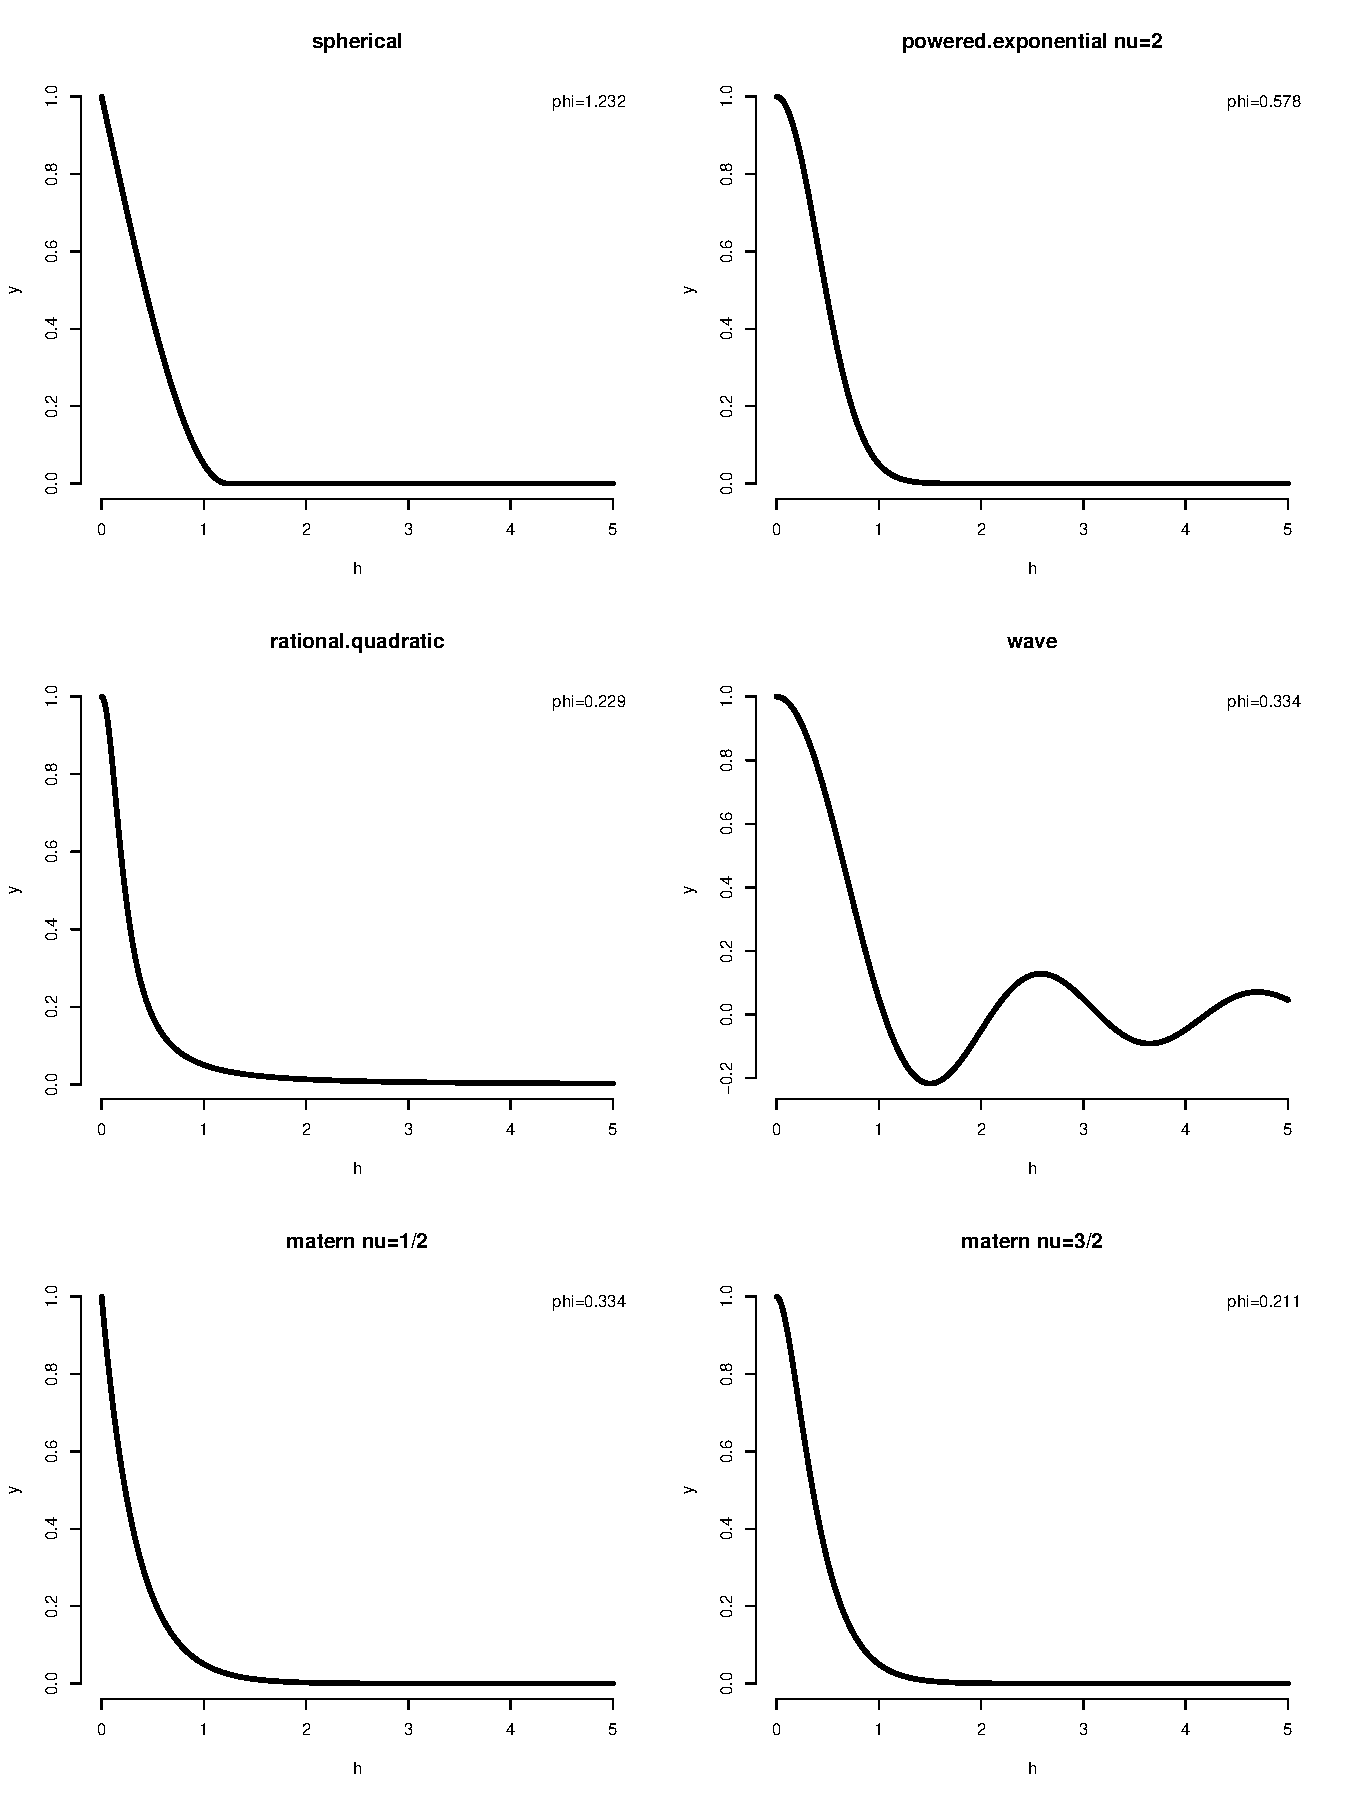
\includegraphics[scale=0.67]{figs/covariance.pdf}
\end{center}

\newpage

Semi-variograms

\begin{center}
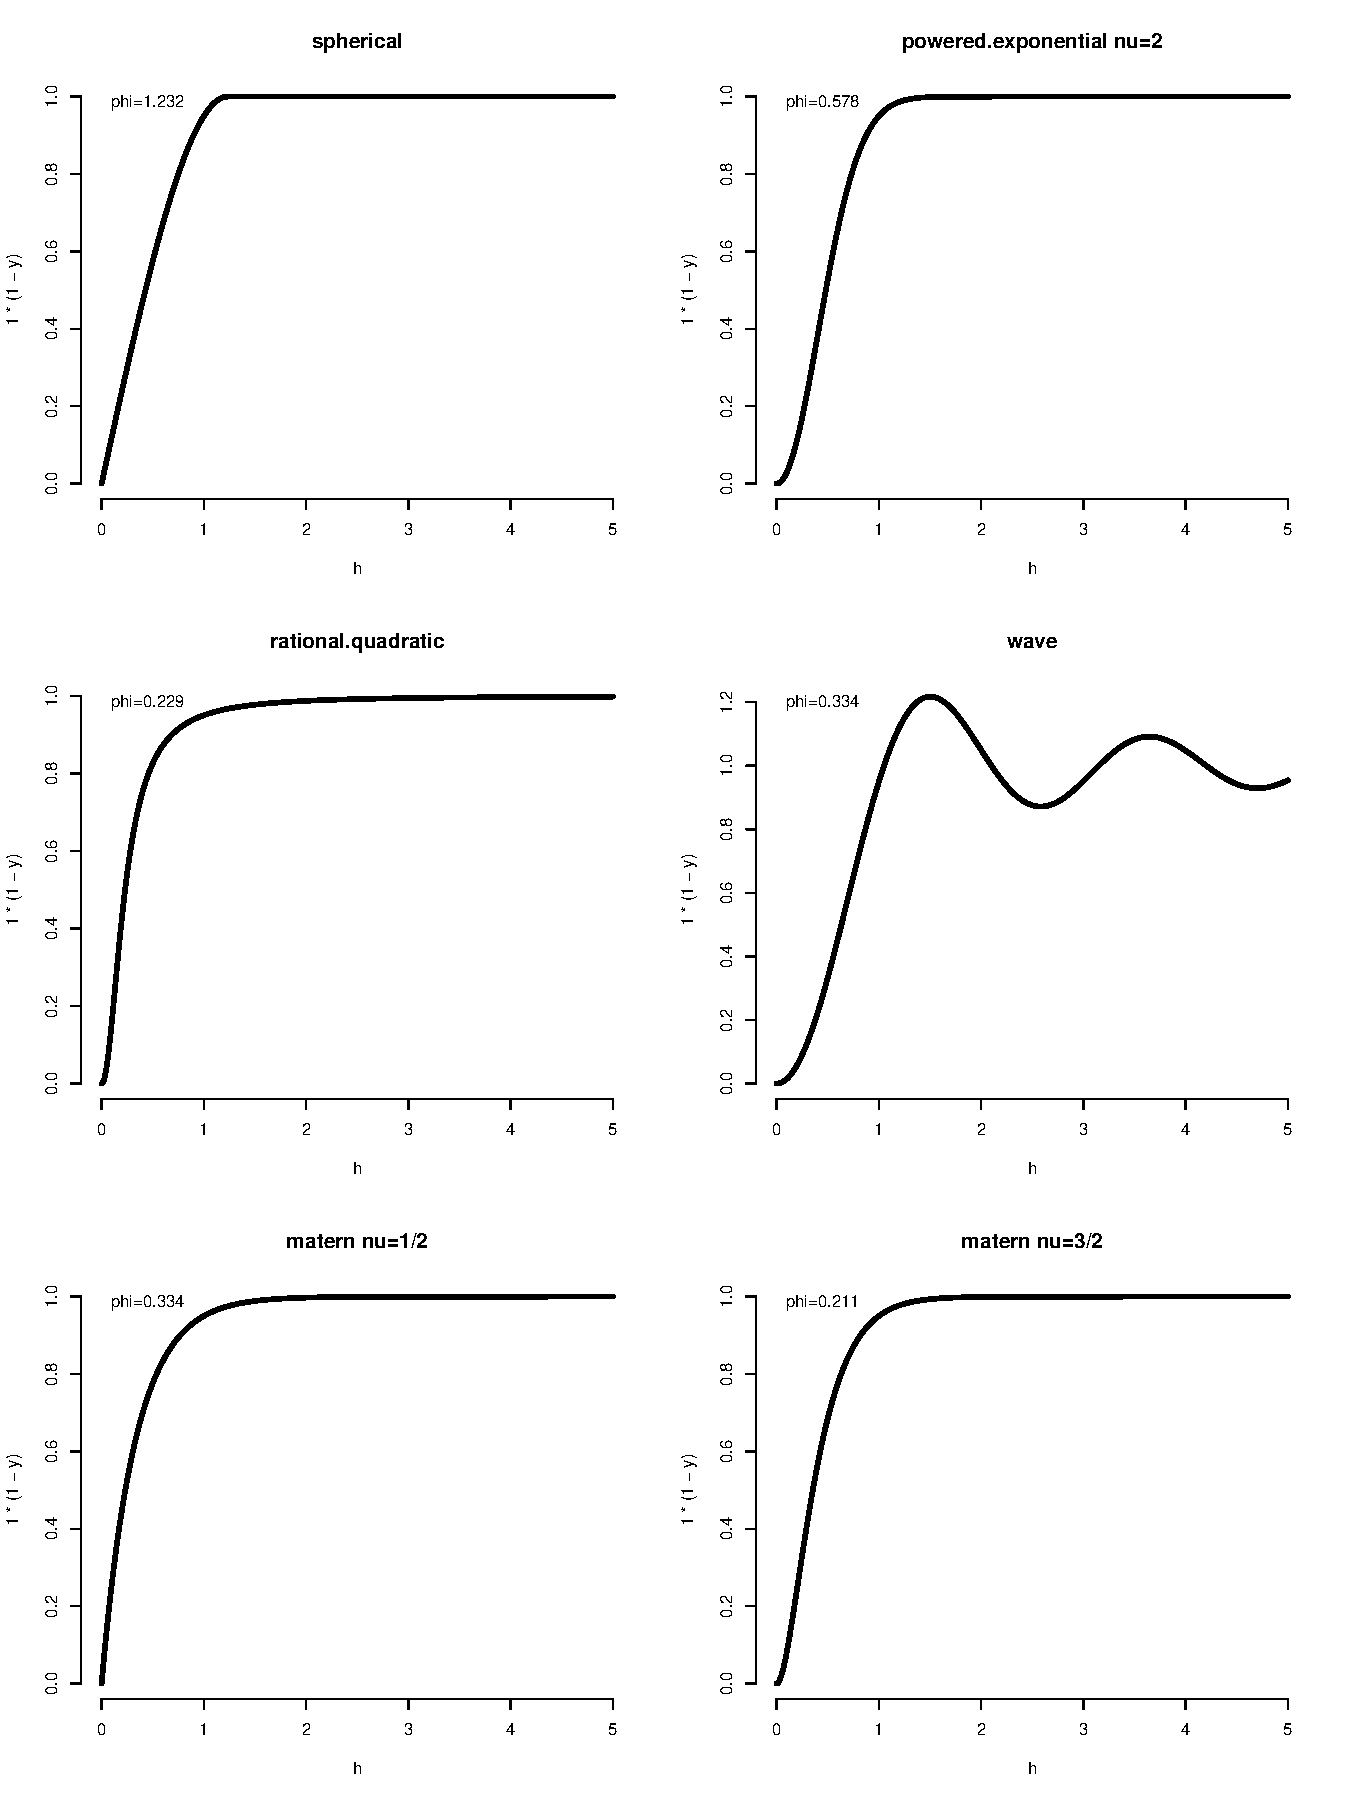
\includegraphics[scale=0.67]{figs/semi-variogram.pdf}
\end{center}

\subsubsection*{4. Assume that the correlation functions in the previous point correspond to one dimensional Gaussian processes. Simulate one 100-points realization of the process corresponding to each of the plotted functions.}

\begin{center}
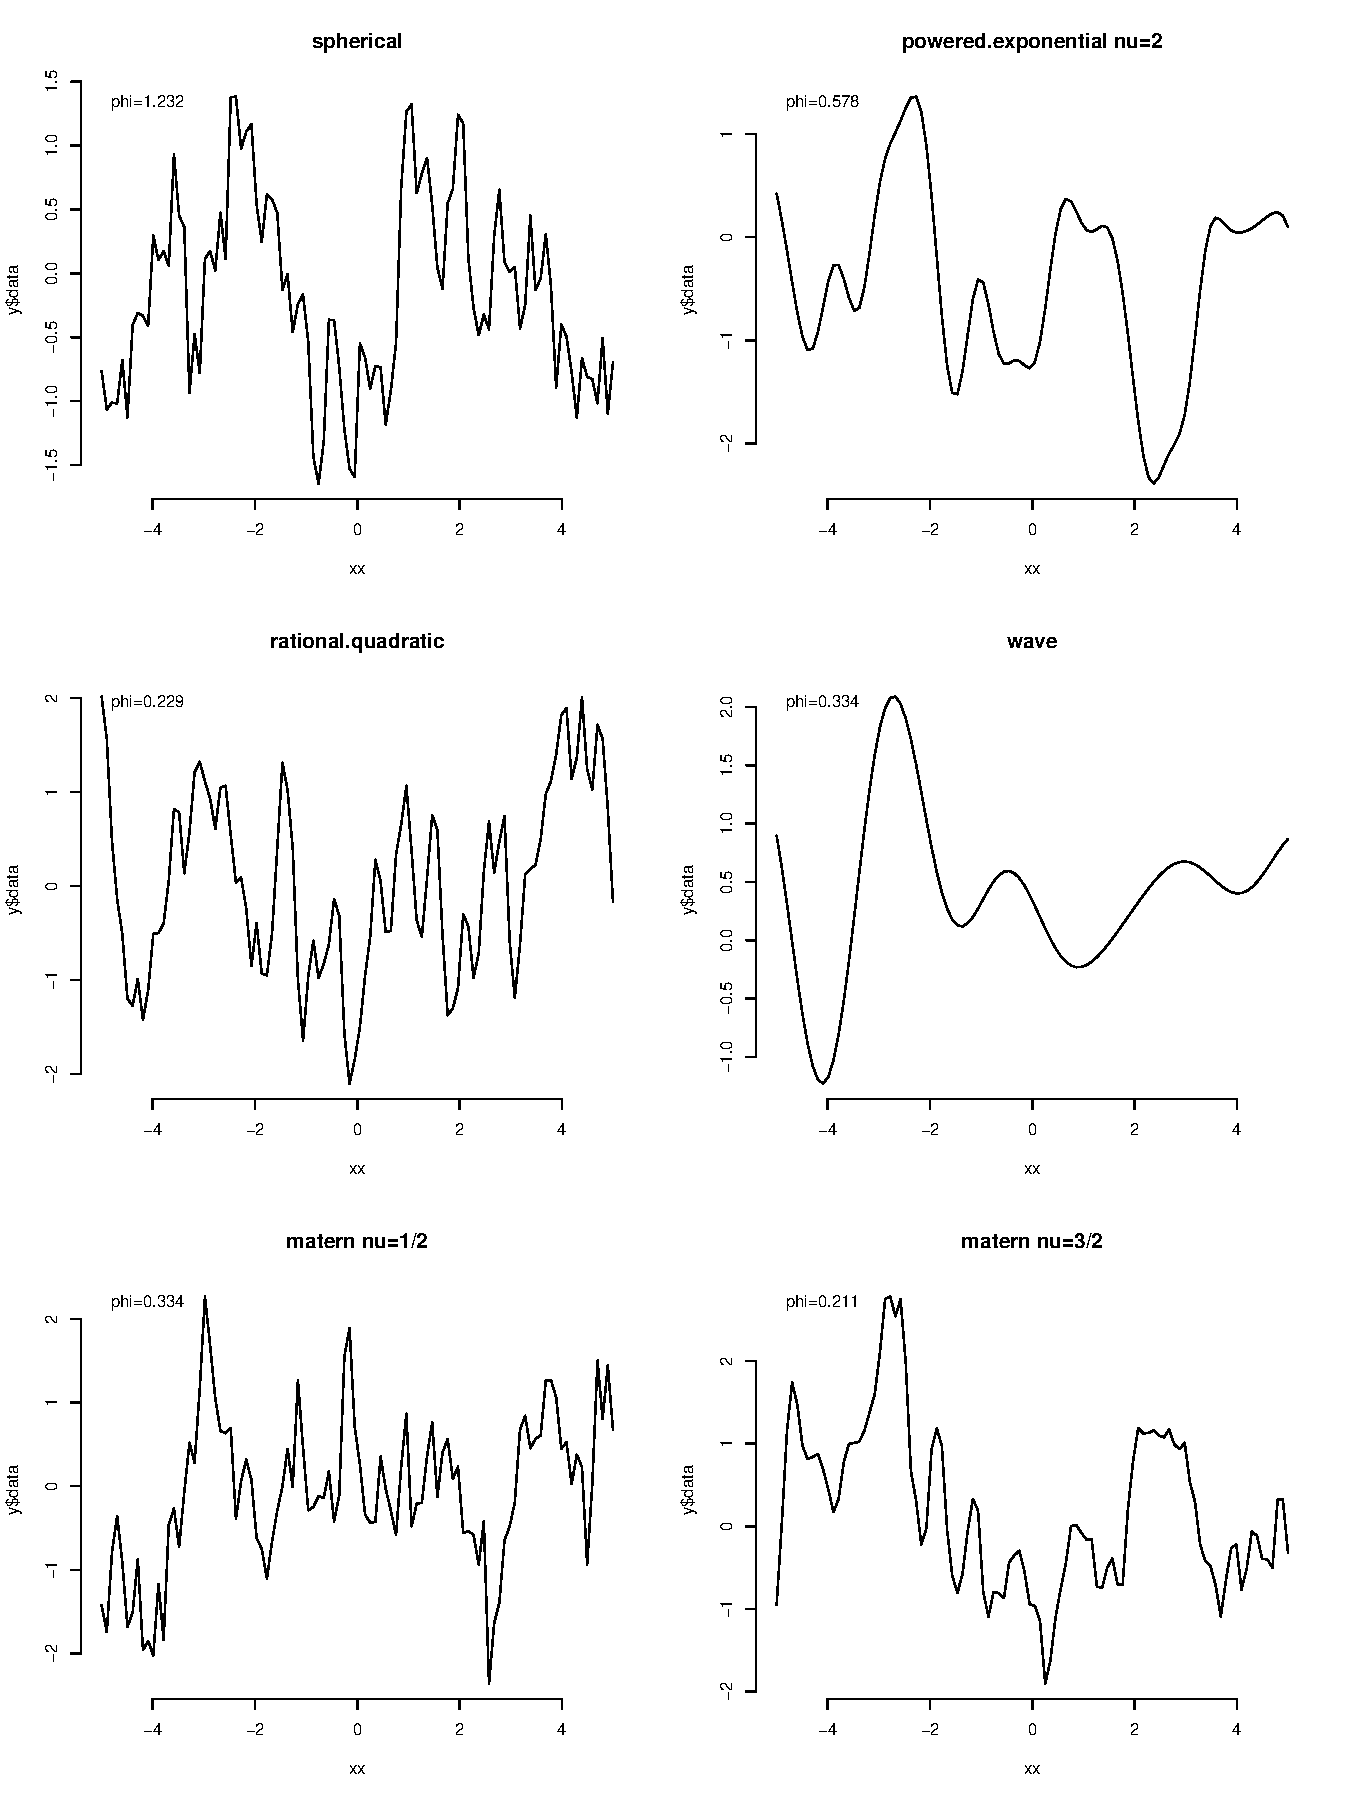
\includegraphics[scale=0.67]{figs/simulations.pdf}
\end{center}

\subsubsection*{5. Write explicitly the correlation function of a Matern with $\nu$=1/2, 3/2, and 5/2.}

\begin{align*}
\rho_{1/2}(\tau) &= \exp\left(-\frac{\tau}{\phi}\right) \\
\rho_{3/2}(\tau) &= \left(1+\frac{\sqrt{3}\tau}{\phi}\right)\exp\left(-\frac{\sqrt{3}\tau}{\phi}\right) \\
\rho_{5/2}(\tau) &= \left(1+\frac{\sqrt{5}\tau}{\phi}+\frac{5\tau^2}{3\phi^2}\right)\exp\left(-\frac{\sqrt{5u}\tau}{\phi}\right) \\
\end{align*}

\end{document}
